\documentclass[conference]{IEEEtran}
\usepackage[T1]{fontenc}
\usepackage{amsmath,amssymb,graphicx,booktabs,array,url}
\usepackage[hidelinks]{hyperref}
\usepackage{placeins}
\usepackage{balance}
\setlength{\emergencystretch}{1em}
\graphicspath{{figures/}}
\title{Criterion: CPU-Only Adaptation and Verified Transformer Inference for Clinical Trial Eligibility Screening}
\author{\IEEEauthorblockN{Muhammad Hashim Rahim}
\IEEEauthorblockA{Student ID: i230028\\FAST NUCES\\Generative AI, Assignment 2}}
\begin{document}
\maketitle
\begin{abstract}
We investigate a locally executable Transformer for criterion-level clinical trial screening on a four-thread CPU without a paid service or GPU. The system adapts SmolLM2-135M-Instruct using low-rank updates and predicts an eligibility category together with patient-sentence evidence. A fixed patient-grouped split prevents patient leakage. We implement explicit key/value-cache decoding, exact greedy speculative decoding with a smaller layer-pruned draft, and educational tiled attention with online softmax. On 206 held-out criteria, adaptation raises accuracy from 23.3\% to 61.2\%, but evidence micro-F1 falls from 0.176 to 0.145; a training-majority reference reaches 62.6\% accuracy. Cached generation reproduces greedy tokens and is 2.02--8.28 times as fast as the uncached reference under the measured settings, while speculation is slower. A standalone browser application supports unseen notes, inclusion/exclusion criteria, source inspection, live inference comparisons and report export. These findings demonstrate CPU feasibility and implementation correctness while exposing substantial reasoning and retrieval failures. Explanations are limited to templates and verbatim model-selected sentences; neither the predictions nor the aggregated trial summary constitute an enrollment decision.
\end{abstract}
\begin{IEEEkeywords}
clinical trial matching, CPU inference, low-rank adaptation, KV cache, online softmax, speculative decoding
\end{IEEEkeywords}

\section{Introduction}
Trial eligibility combines clinical facts, logical conditions and incomplete records. A positive inclusion requirement and a disqualifying exclusion condition have different semantics. A missing fact cannot safely establish either eligibility or ineligibility. This project therefore predicts each criterion separately and preserves the expert categories, including insufficient information and non-applicability.

The assignment is treated as a research and implementation task, not a reproduction of an existing application. The contributions are a CPU-executable supervised pipeline, three independently implemented autoregressive decoding paths, a numerically checked tiled-attention implementation, and a browser interface that exposes evidence and measured behavior. Evaluation concerns the criterion-level benchmark. An overall screening message is only an explicit rule applied to the supplied criteria.

\section{Related Work and Design Alternatives}
TrialGPT separates retrieval, criterion matching and aggregation \cite{trialgpt}. Its criterion annotations provide expert labels and evidence locations used here. We implement a smaller supervised matcher and do not copy its model predictions or claim its published performance. A compact model trades reasoning capacity for local feasibility \cite{smol}. The two architecture candidates in Table~\ref{tab:models} share a Llama-style decoder architecture and tokenizer family, but require different weight memory.

LoRA freezes pretrained matrices and learns low-rank residual updates \cite{lora}. We choose it over full adaptation to reduce optimizer state and trainable memory. Adapting only the last six blocks further limits backward propagation through early blocks, at the cost of adaptation capacity. We do not assume LoRA alone eliminates activation memory or CPU computation.

KV caching reuses historical keys and values across generation steps; positions and attention-mask dimensions must still account for the entire prefix \cite{cache}. FlashAttention motivates attention tiling and stable incremental normalization \cite{flash}. Our educational PyTorch implementation uses these mathematical ideas, without implementing its fused accelerator kernel or claiming equivalent hardware speed.

Speculative decoding uses a draft to propose multiple tokens for target verification \cite{spec}. We implement its deterministic greedy specialization: accept exactly the target's matching prefix and correct the first mismatch. Unlike distribution-preserving stochastic speculative sampling, this experiment only claims greedy token equivalence. A pruned draft is feasible in RAM but can have poor acceptance. This is a measured limitation, not an assumed acceleration.

\section{Materials and Methods}
\subsection{Dataset Integrity and Fixed Split}
The sole supervised source is the TrialGPT Criterion Annotations dataset \cite{dataset}. It contains 1,015 criterion annotations over 53 patients. We sort unique patient IDs, shuffle them with NumPy \texttt{default\_rng(42)}, and assign the first 37 patients to training, the next eight to validation and the final eight to testing. Table~\ref{tab:split} reports the resulting counts. Patient IDs, annotation counts and the raw-file checksum are saved in the manifest.

\begin{table}[t]\centering
\caption{Patient-grouped benchmark partition. All rows for a patient remain together.}\label{tab:split}
\begin{tabular}{lrr}\toprule Partition & Patients & Criteria\\\midrule
Train & 37 & 603\\ Validation & 8 & 206\\ Test & 8 & 206\\\bottomrule\end{tabular}
\end{table}

Preprocessing explicitly whitelists identifiers, patient text, criterion type/text, expert eligibility and expert evidence. Previous GPT explanations, predictions, sentence selections, annotation-quality judgments and the source training flag are excluded. Identifiers are retained for auditing but not included in the model prompt. Global schema and split-integrity checks do not guide model selection. Test predictions are generated only after the checkpoint and source-code hashes are frozen.

\subsection{Inputs, Outputs and Truncation}
Original numbered sentences keep their dataset IDs. Unnumbered application notes are split deterministically and numbered from zero. The input consists of a task instruction, the permitted labels for the criterion type, the numbered record, and the criterion. The label vocabulary is
\{included, not included, excluded, not excluded, not enough information, not applicable\}. Inclusion permits the first two and last two labels; exclusion permits the middle two and last two.

For CPU efficiency, the autoregressive response is one single-token label code followed by a binary evidence flag for each retained sentence, in original order. A deterministic parser returns a JSON label, original sentence IDs and verbatim text. The bitmap can represent any evidence subset, including an empty set. Greedy decoding masks the label vocabulary at the first step and permits only binary tokens thereafter. This same grammar is used before and after adaptation; it is an explicit structured-output constraint, not a clinical rule or a gold-label feature.

The total input plus response budget is 1,024 tokens. Complete leading sentences are retained while whole trailing sentences are removed if necessary. Gold evidence never selects the retained window. Omitted sentence IDs and omitted gold citations are logged. No evidence is silently renumbered. Extremely long criteria or records without a fitting complete sentence are rejected. Table~\ref{tab:training} and the generated results describe observed truncation.

\subsection{Model and Low-Rank Adaptation}
\begin{table}[t]\centering\small
\caption{Open-weight model candidates. Float32 weight estimates exclude activations, optimizer, cache and framework overhead. Both use Apache-2.0 licensing and an 8,192-token configured context.}\label{tab:models}
\setlength{\tabcolsep}{4pt}\begin{tabular}{lrr}\toprule & 135M selected & 360M alternative\\\midrule
Decoder blocks & 30 & 32\\Hidden width & 576 & 960\\Query/KV heads & 9/3 & 15/5\\Head dimension & 64 & 64\\Vocabulary & 49,152 & 49,152\\Nominal FP32 weights & 0.54 GB & 1.44 GB\\\bottomrule\end{tabular}
\end{table}
SmolLM2-135M-Instruct uses rotary positions, grouped-query attention, RMS normalization, SwiGLU-style feed-forward blocks and tied input/output embeddings \cite{smol,config135,config360}. We execute float32 eager attention on CPU. The model cards identify the licensing, while the downloaded configurations establish architectural sizes. The exact base revision is pinned in the download script.

For the final six blocks, query and value projections become
\begin{equation} y = Wx + (\alpha/r) BAx, \qquad r=8,\quad\alpha=16. \end{equation}
The base matrices are frozen. $A$ is Kaiming-initialized and $B$ starts at zero, preserving base behavior before optimization. We train 92,160 adapter parameters with AdamW, learning rate $10^{-3}$, gradient norm clipping at 1 and effective batch size eight through gradient accumulation. Each example has batch size one. Training uses three fixed epochs, seed 42, and response-only next-token cross entropy. The final partial accumulation group uses its actual size. Minimum token-weighted validation loss selects the checkpoint; test performance cannot select it.

The output projection is evaluated only for hidden positions needed to predict the response. This avoids allocating prompt-length vocabulary logits while preserving the response loss. A development check compares it numerically with the library's fully projected masked loss. The frozen early blocks still execute; computational savings are not presented as zero-cost training.

Two engineering alternatives were tested during development. Full prompt-logit projection and response-only projection agreed to approximately $10^{-6}$ on the checked masked loss; their single-example timings are retained as a development check, not a controlled benchmark. The initial spaced-digit output format used two tokenizer tokens per flag. We replaced that assumption with explicit single-digit token construction and asserted the resulting response length. The plain completion prompt was retained identically for base and adapted evaluation; no clinical prompt or threshold was selected using test cases.

\subsection{Evidence and Explanation Pipeline}
The label code and bitmap are translated without label collapsing. Each citation is guaranteed to refer to a retained source sentence, although this does not guarantee medical relevance. The explanation uses a fixed description of the prediction and verbatim cited text, avoiding a second unconstrained rationale generation. Empty evidence triggers review regardless of the predicted label. Insufficient information and truncation also trigger review. This conservative review flag does not replace the model's label when calculating benchmark metrics.

The trial summary applies the following precedence: any predicted exclusion or failed inclusion yields a potential conflict; otherwise missing information, missing evidence or non-applicability requests review; otherwise the supplied criteria have no predicted conflict. These are application rules, not learned or benchmark-labeled trial outcomes. All paths require human verification.

\subsection{Explicit Cache-Aware Generation}
The uncached reference recomputes the full prompt and generated prefix at every step. The cached path prefills once into a dynamic cache and subsequently forwards only the newest token. The attention mask spans the past and current tokens; absolute rotary position indices start at the cache length. The cache grows by one token per incremental forward. The final emitted token need not be forwarded again when generation stops. Cache-length traces are stored for verification.

Both paths use argmax with identical structured constraints when screening. Benchmarks use unrestricted greedy generation at fixed output lengths to avoid response-length confounding. Different matrix shapes can introduce floating-point differences even for mathematically equivalent computations, so token equality is tested rather than assumed. Failed equality must stop an experiment instead of being hidden by an aggregate timing result.

\subsection{Tiled Attention with Online Softmax}
The dense reference calculates
\begin{equation} O = \operatorname{softmax}(QK^\top/\sqrt{d}+M)V, \end{equation}
where $M$ is zero for visible keys and negative infinity for masked keys. Its stable implementation subtracts each row maximum before exponentiation.

For each query tile, the tiled version initializes a running maximum $m=-\infty$, normalizer $l=0$ and unnormalized output $a=0$. For a score tile $S$, it updates
\begin{align}
m'&=\max(m,\operatorname{rowmax}(S)),\\
P&=\exp(S-m'),\quad s=\exp(m-m'),\\
l'&=s l+\operatorname{rowsum}(P),\\
a'&=s a+PV_{\mathrm{tile}},\quad O=a/l.
\end{align}
All-masked tiles contribute zero rather than producing NaNs from $-\infty-(-\infty)$. Causal comparisons use absolute query/key indices and support a query offset for rectangular attention. Tests cover unequal dimensions, non-divisible tiles, causal/noncausal masks and an offset. The default score tile is $32\times32$. No fused attention operator implements either reference or tiled calculation. The educational implementation is tested separately; it does not replace the target model's eager attention.

\subsection{Greedy Speculative Decoding}
The smaller draft retains the first six blocks and shared tokenizer definition of the base 135M model. It has 49,552,704 parameters (approximately 189.0 MiB of float32 weights), compared with 134,515,008 base target parameters (513.1 MiB). It is an uncalibrated layer-pruned language model, not an independently pretrained smaller model. Its original pretrained embeddings, layers and final normalization are reused. Target adaptation is not applied to the draft. This explicit construction avoids an incompatible-tokenizer pair and a second large download, but early-layer pruning can severely reduce proposal quality.

Each round begins with both caches representing the accepted prefix and logits predicting its successor. The draft greedily proposes up to four tokens. A single target forward verifies their block. The saved pre-block target logits verify candidate zero; block logit $j-1$ verifies candidate $j$. The algorithm accepts the matching prefix. At a mismatch it crops both caches to that prefix and forwards the target's corrective token through both models. If all candidates match, it may emit one bonus target token and synchronize both caches. Cache-length assertions check every completed round. End-of-sequence and output-budget boundaries are handled explicitly. Greedy equality tests exercise rejection, complete acceptance, grammar constraints and early stopping.

\subsection{Browser Application}
The Flask application binds to loopback and opens the browser through a double-click launcher. The evaluator enters a note and one or more criteria or selects training-set trial metadata. Requests run sequentially through a worker queue; input errors and model-loading failures are displayed. Patient records are kept in process memory, excluded from experiment logs and not sent to a remote inference service. The app shows each criterion label, citation text, truncation warning and elapsed time. HTML export is escaped and printable. The inference lab runs a live three-mode comparison, and the study view reads the actual saved results. Appendix materials provide startup and demonstration instructions.

\section{Experimental Setup and Metrics}
The experiment uses Windows, Python 3.13.5, four available logical CPU threads and approximately 7.89 GiB RAM. PyTorch uses two intra-operation threads. Dependency versions and hardware details are recorded. Base weights, tokenizer revision, seed, split manifest, training configuration and selected adapter are supplied or reproducibly downloadable. CPU-only execution is compulsory for this implementation; no GPU result is claimed.

Training wall time includes concurrent base-validation work during the early part of the run. It is an observed execution duration, not an isolated training-throughput comparison. Final inference and attention benchmarks run sequentially after these jobs have finished.

We report criterion accuracy, macro-F1 over the full applicable label vocabulary (including zero-support labels with zero division set to zero), per-class precision/recall/F1, and confusion matrices overall and by criterion type. Evidence is evaluated as sets of original sentence IDs. Micro scores pool TP/FP/FN; macro scores average per-record precision, recall and F1. A pair of empty gold/predicted sets scores one per record and contributes no micro counts; exactly one empty set scores zero. Full untruncated gold sets are used, so dropped evidence would count as a false negative.

Decoding benchmarks use three input/output pairs: 32/8, 128/16 and 256/32 tokens, the same adapted target and identical prompts. Each configuration runs in a fresh subprocess, gets one warmup and three measured repetitions. CPU operations complete synchronously; no CUDA synchronization is applicable. We record prefill, subsequent decode time, total time, throughput and process peak resident memory. Prefill in speculative mode includes both models. Total throughput divides emitted tokens by end-to-end time; decode-only timing excludes prefill. Peak RSS includes interpreter, weights, warmup and tensor buffers, not just cache allocations. These measurements are taken after training/evaluation completes to reduce contention.

Attention uses float32 tensors with batch one, three heads, head width 32 and sequence lengths 64--512. We report maximum/mean absolute numerical errors, repeated CPU latency, score-buffer estimates and fresh-process peak RSS. RSS is sampled before allocating the independent dense output used for numerical verification. Allocator high-water behavior and interpreter memory can obscure small tensor-memory differences.

\section{Results and Discussion}
\begin{figure*}[t]\centering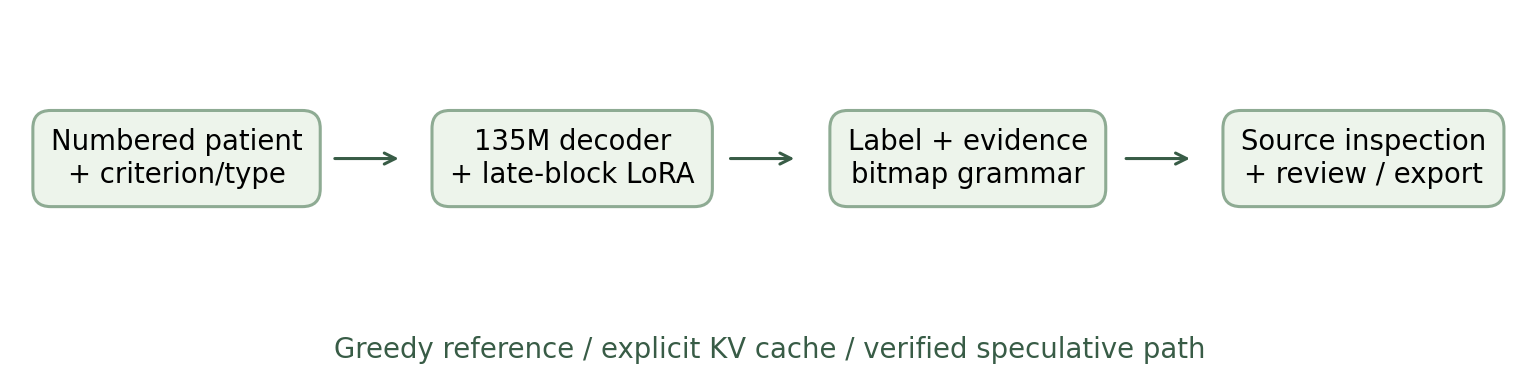
\includegraphics[width=\textwidth]{workflow.png}\caption{Screening workflow. All decoding modes share the target model; the evidence parser preserves source sentence IDs.}\label{fig:workflow}\end{figure*}

Figure~\ref{fig:workflow} summarizes the application path. The full experiments use 603 training annotations; development smoke runs are archived separately and are not reported as final results.

The original CPU automated suite reports 16 passing checks. These cover attention agreement, cached/uncached/speculative token equality, cache growth, full-acceptance and rejection branches, early stopping, structured masks, evidence empty-set conventions, data isolation, response-loss equivalence, frozen base weights, truncation and application input/export handling.

\begin{table}[t]\centering\small\caption{Selected training configuration and observed preprocessing.}\label{tab:training}\begin{tabular}{lr}\toprule Setting & Value\\\midrule

Target parameters & 134,607,168\\

Trainable parameters & 92,160\\

Selected epoch & 3\\

Best validation loss & 0.3446\\

Three-epoch elapsed time & 55.13 min\\

Train truncated records & 0\\

Validation truncated records & 0\\

Test truncated records & 0\\\bottomrule\end{tabular}\end{table}

\begin{figure}[t]\centering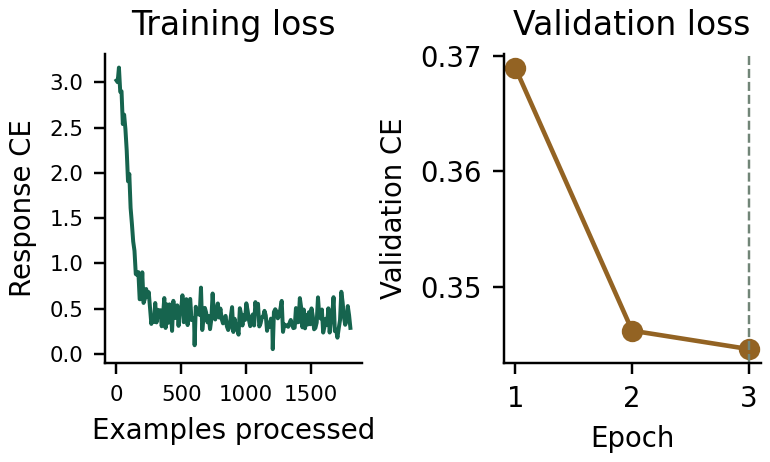
\includegraphics[width=\columnwidth]{training.png}\caption{Measured training and validation response loss. The dashed line marks the selected epoch.}\label{fig:training}\end{figure}

Table~\ref{tab:training} records the selected adapter. Validation loss changed from 0.3690 after epoch one to 0.3446 after epoch three (Fig.~\ref{fig:training}). Selection uses the minimum validation loss, not the final test score. Training loss windows are descriptive and are not an unbiased epoch-average curve.

\begin{table}[t]\centering\small\caption{Validation comparison. Acc=accuracy; MF=macro-F1; EF=evidence micro-F1.}\label{tab:validation}\begin{tabular}{llrrr}\toprule Model & Criteria & Acc & MF & EF\\\midrule

base & overall & 0.199 & 0.148 & 0.157\\

base & inclusion & 0.530 & 0.177 & 0.417\\

base & exclusion & 0.043 & 0.047 & 0.093\\

adapted & overall & 0.641 & 0.273 & 0.155\\

adapted & inclusion & 0.470 & 0.234 & 0.234\\

adapted & exclusion & 0.721 & 0.210 & 0.000\\

\bottomrule\end{tabular}\end{table}

\begin{table}[t]\centering\small\caption{Held-out comparison. Acc=accuracy; MF=macro-F1; EF=evidence micro-F1.}\label{tab:test}\begin{tabular}{llrrr}\toprule Model & Criteria & Acc & MF & EF\\\midrule

base & overall & 0.233 & 0.155 & 0.176\\

base & inclusion & 0.347 & 0.135 & 0.305\\

base & exclusion & 0.168 & 0.099 & 0.096\\

adapted & overall & 0.612 & 0.259 & 0.145\\

adapted & inclusion & 0.467 & 0.220 & 0.196\\

adapted & exclusion & 0.695 & 0.205 & 0.000\\

\bottomrule\end{tabular}\end{table}

Tables~\ref{tab:validation} and~\ref{tab:test} compare identical examples and grammar settings before and after adaptation. Held-out accuracy changes from 0.233 to 0.612, while macro-F1 changes from 0.155 to 0.259. These measures must be interpreted together: frequent-label success can raise accuracy while rare classes remain poorly recognized. The results do not establish clinical reliability.

A diagnostic majority-label reference chooses the most frequent training label separately for each criterion type, with no test-derived choice. It obtains held-out accuracy 0.626 and macro-F1 0.226. This simple reference contextualizes the adapted model: improvement over an unadapted decoder does not by itself demonstrate strong clinical discrimination. The reference performs no evidence retrieval.

Evidence micro-F1 changes from 0.176 before adaptation to 0.145 afterwards. A label-accuracy gain therefore must not be described as a general evidence-quality gain. Many zero evidence flags and imbalanced label frequencies are plausible contributors, but this study does not establish their causal effect through an ablation.

The actual prediction distribution is inclusion: included (21), not enough information (54); exclusion: not excluded (131). No sentence was cited in 181 of 206 test records. Thus syntactic preservation of all six labels must not be confused with successful recognition of all six classes. The concentration on frequent outcomes and weak evidence selection are substantive failures of the adapted matcher. Verified inference mechanisms do not establish clinical reasoning quality.

\begin{table}[t]\centering\scriptsize\caption{Adapted model: held-out per-class classification. All six labels remain distinct.}\label{tab:classes}\begin{tabular}{lrrrr}\toprule Label & Prec. & Recall & F1 & N\\\midrule

included & 0.286 & 0.222 & 0.250 & 27\\

not included & 0.000 & 0.000 & 0.000 & 7\\

excluded & 0.000 & 0.000 & 0.000 & 0\\

not excluded & 0.695 & 1.000 & 0.820 & 91\\

not enough information & 0.537 & 0.439 & 0.483 & 66\\

not applicable & 0.000 & 0.000 & 0.000 & 15\\

\bottomrule\end{tabular}\end{table}

\begin{figure*}[t]\centering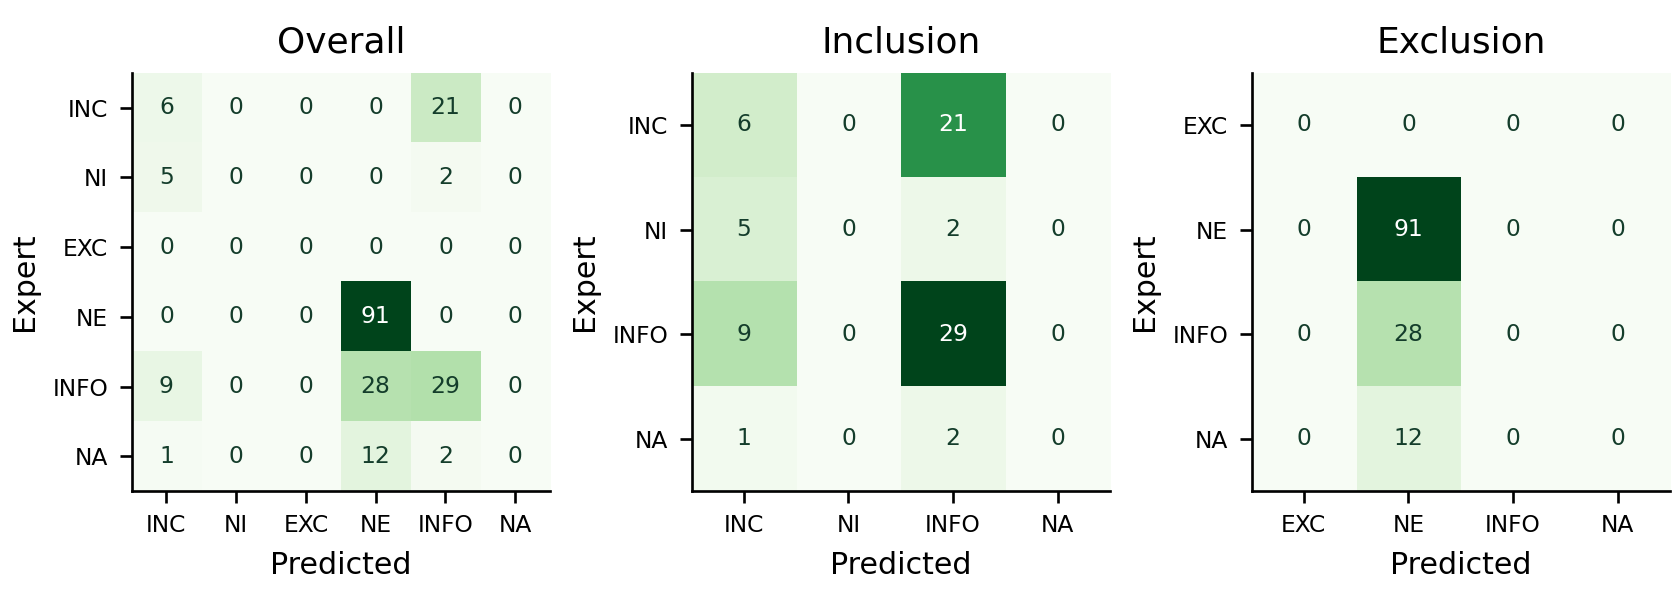
\includegraphics[width=\textwidth]{confusion.png}\caption{Adapted held-out confusion matrices. Rows are expert labels and columns are predictions. INC=included; NI=not included; EXC=excluded; NE=not excluded; INFO=not enough information; NA=not applicable.}\label{fig:confusion}\end{figure*}

Table~\ref{tab:classes} and Fig.~\ref{fig:confusion} expose minority-class errors that overall accuracy obscures. Zero-support classes remain in the specified macro denominator. Per-type per-class results and both base/adapted confusion matrices are also saved in the machine-readable metric files.

\begin{table}[t]\centering\scriptsize\caption{Adapted held-out evidence retrieval. Both-empty pairs score one per record, but contribute no pooled counts.}\label{tab:evidence}\begin{tabular}{lrrrrrr}\toprule & \multicolumn{3}{c}{Micro} & \multicolumn{3}{c}{Macro}\\Group & P & R & F1 & P & R & F1\\\midrule

overall & 0.300 & 0.096 & 0.145 & 0.690 & 0.694 & 0.691\\

inclusion & 0.300 & 0.145 & 0.196 & 0.362 & 0.373 & 0.364\\

exclusion & 0.000 & 0.000 & 0.000 & 0.878 & 0.878 & 0.878\\

\bottomrule\end{tabular}\end{table}

Table~\ref{tab:evidence} includes 134 test records where both evidence sets are empty. Differences between micro and macro scores reflect both citation-set sizes and the explicit empty-set convention. Evidence scores assess localization; they do not prove that cited sentences logically entail the model label.

\begin{table*}[t]\centering\small\caption{Adapted CPU decoding measurements. Median of three repetitions after one warmup; peak RSS is a fresh-process high-water mark including loaded model(s).}\label{tab:decode}\begin{tabular}{rrlrrrrr}\toprule Input & Output & Path & Prefill (s) & Decode (s) & Total (s) & Tokens/s & Peak RSS (MiB)\\\midrule

32 & 8 & uncached & 0.212 & 1.278 & 1.481 & 5.40 & 1206.2\\

32 & 8 & cached & 0.140 & 0.576 & 0.732 & 10.92 & 1206.2\\

32 & 8 & speculative & 0.183 & 2.407 & 2.591 & 3.09 & 1748.4\\

128 & 16 & uncached & 0.375 & 6.694 & 7.051 & 2.27 & 1206.9\\

128 & 16 & cached & 0.401 & 1.523 & 1.945 & 8.23 & 1206.8\\

128 & 16 & speculative & 0.520 & 5.044 & 5.644 & 2.83 & 1748.1\\

256 & 32 & uncached & 0.884 & 31.163 & 32.212 & 0.99 & 1206.7\\

256 & 32 & cached & 0.859 & 3.012 & 3.891 & 8.22 & 1206.1\\

256 & 32 & speculative & 1.019 & 10.878 & 12.126 & 2.64 & 1748.5\\

\bottomrule\end{tabular}\end{table*}

\begin{figure}[t]\centering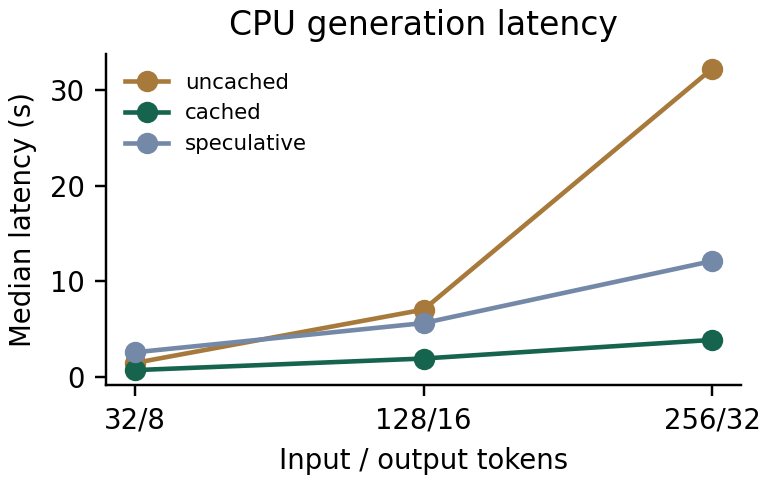
\includegraphics[width=\columnwidth]{latency.png}\caption{Measured end-to-end generation latency, including prefill.}\label{fig:latency}\end{figure}

Token-level agreement across all three final length pairs is verified. Table~\ref{tab:decode} and Fig.~\ref{fig:latency} separate prefill from incremental decoding. Caching avoids repeated prefix computation but retains KV memory. Process RSS includes fixed framework and weight costs, so it is not an isolated cache-size measure.

Across the measured length pairs, cached generation is 2.02--8.28 times as fast as the uncached reference by median end-to-end latency. These ratios apply to this target, CPU, prompt family and output budgets; they are not universal model speedups.

\begin{table}[t]\centering\scriptsize\caption{Speculative acceptance and speed relative to ordinary cached greedy. Speedup below one means slower.}\label{tab:spec}\begin{tabular}{rrrr}\toprule Input/output & Accepted/proposed & Acceptance & Speedup\\\midrule

32/8 & 0/26 & 0.000 & 0.283\\

128/16 & 2/54 & 0.037 & 0.345\\

256/32 & 2/114 & 0.018 & 0.321\\

\bottomrule\end{tabular}\end{table}

Table~\ref{tab:spec} reports proposal counts from the first deterministic run and the median latency ratio. Low acceptance requires repeated draft forwards and target corrections. A smaller model is therefore insufficient by itself to guarantee acceleration. The pruned draft is a practical memory experiment with limited calibration, and the measured ratios bound claims about its usefulness.

\begin{table}[t]\centering\scriptsize\caption{Educational attention measurements (batch 1, heads 3, width 32). Error is against the dense reference.}\label{tab:attention}\begin{tabular}{rlrrr}\toprule Length & Path & Time (ms) & Max error & RSS MiB\\\midrule

64 & reference & 0.302 & 0.0e+00 & 395.1\\

64 & tiled & 1.986 & 3.6e-07 & 395.5\\

128 & reference & 1.425 & 0.0e+00 & 396.3\\

128 & tiled & 9.197 & 3.0e-07 & 395.6\\

256 & reference & 2.307 & 0.0e+00 & 398.9\\

256 & tiled & 17.209 & 6.0e-07 & 396.2\\

512 & reference & 7.926 & 0.0e+00 & 412.7\\

512 & tiled & 84.642 & 4.8e-07 & 396.2\\

\bottomrule\end{tabular}\end{table}

Table~\ref{tab:attention} shows a maximum tiled numerical error of 5.96e-07; the largest mean error is 2.79e-08. The logical score tile stays at most 0.0117 MiB, whereas the dense score tensor reaches 3.00 MiB. These buffer estimates exclude other intermediates and are not claimed as peak process-memory savings. Python loops and small tensor dispatch can outweigh tiling benefits on CPU.

At sequence length 512, the tiled implementation takes 84.642 ms versus 7.926 ms for dense attention. This directly measures the educational implementation, not a fused FlashAttention kernel.

\begin{table*}[t]\centering\scriptsize\caption{Eight distinct adapted-model held-out error cases. Full notes, IDs, gold and predicted evidence are preserved in the error-analysis file.}\label{tab:errors}\begin{tabular}{rp{4.4cm}p{2.1cm}p{2.1cm}p{4.2cm}}\toprule ID & Criterion (abbreviated) & Expert label & Prediction & Observed error\\\midrule

160 & Patient willing to give full informed consent for participation & included & included & extra citation, missed citation\\

161 & Patients undergoing elective carotid endarterectomy & not included & included & missed inclusion conflict, extra citation\\

165 & Pregnancy & not applicable & not excluded & applicability confusion\\

169 & Patients with an estimated pre-operative glomerular filtration rate \(<\) 30mls/min/1.73m2 & not enough information & not excluded & unsupported certainty\\

179 & Had been performed central venous puncture or catheterization before. & not excluded & not excluded & missed citation, empty predicted evidence\\

185 & Patients were included if they were diagnosed with Shock, Acute respiratory distress syndrome (ARDS), or both. & included & not enough information & over-abstention, missed citation, empty predicted evidence\\

304 & Patients of both sexes aged \(\geq\) 18 years. & included & not enough information & over-abstention, missed citation, empty predicted evidence\\

381 & Age \(>\) 18 years at the time of signing the informed consent form & included & not enough information & over-abstention, missed citation, empty predicted evidence\\

\bottomrule\end{tabular}\end{table*}

Table~\ref{tab:errors} distinguishes label errors from sentence-localization errors. Unsupported certainty is defined relative to an expert insufficient-information label, not an independently established medical diagnosis. Extra/missed citations compare source-ID sets. The cases show why a valid citation ID and a grammatical output cannot establish factual support. The full error log retains contradictory expert/model outcomes and source text for individual review.

Annotation 161 is an unsupported positive result: the criterion specifies elective carotid endarterectomy, whereas cited sentence 0 describes cardiac catheterization. The citation is a valid source location but does not state the required procedure. This demonstrates the gap between source-ID validity and criterion entailment.

Annotation 169 asks about a pre-operative renal-filtration threshold. The supplied note contains no such measurement. The expert label is insufficient information, but the model returns not excluded with no citation. The app flags the absent evidence for review; the predicted negative outcome must not be read as proof that the threshold is not met.

Annotation 185 combines under-recognition and failed localization. The experts associate the inclusion criterion with sentences 2 and 3, which report observations and vital signs; the model instead abstains and retrieves neither sentence. The error concerns the benchmark expert judgment, not an independent clinical diagnosis made by this system.

\begin{table}[t]\centering\scriptsize\caption{Supplementary synthetic probes. These are not benchmark labels and are excluded from accuracy/F1.}\label{tab:stress}\begin{tabular}{p{2.5cm}p{3.1cm}l}\toprule Probe & Model output & Cited IDs\\\midrule

Conflicting ages & not enough information & []\\

Missing kidney data & not excluded & []\\

Explicit negation & included & [0]\\

\bottomrule\end{tabular}\end{table}

Table~\ref{tab:stress} tests three deliberately constructed situations after protocol freeze. The conflicting-age record contains both 52 and 72 years without resolving the discrepancy; citing a single age cannot resolve that contradiction. The missing-kidney-information case provides no renal measurement; a definite category would not establish that missing fact. The negation case distinguishes a condition mention from its presence. These probes illustrate behaviors for human review, not additional ground-truth benchmark performance or a basis for retuning.

\subsection{Final Browser Workflow Verification}

\begin{figure*}[t]\centering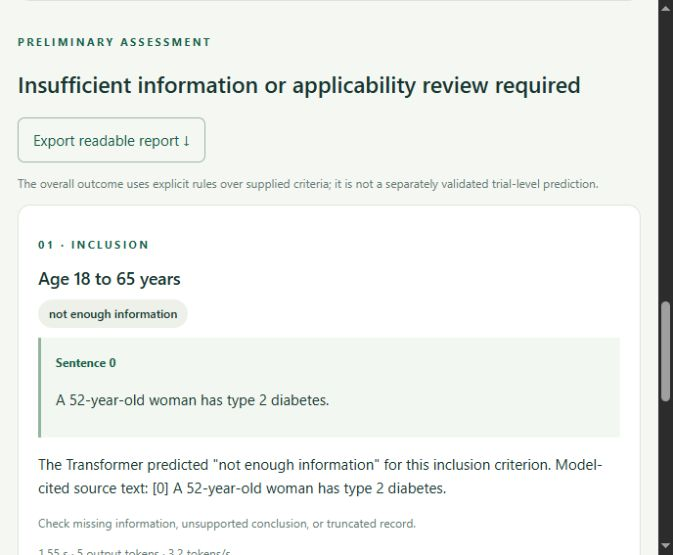
\includegraphics[width=\textwidth]{application.jpg}\caption{Genuine browser capture of the final CPU application on a synthetic record. The model abstains on an age criterion despite citing the stated age; this visible failure is preserved. The review warning and report-export control are part of the running interface.}\label{fig:app}\end{figure*}

Figure~\ref{fig:app} shows an actual model result, not a mockup. Empty-note and malformed-criterion errors were displayed, followed by successful recovery. Cached, uncached and speculative screening completed through browser controls with identical emitted tokens. The downloaded HTML report was opened in a browser and retained the synthetic record, citation, selected epoch and adapter fingerprint. The study-results tab displayed the saved held-out metrics. These functional checks do not validate clinical reasoning.

A browser-triggered live comparison used 151 input tokens and 16 raw output tokens, one warmup and two measured repeats per mode. Token equality passed. Mean total latency was 7.489 s uncached, 1.785 s cached, and 5.916 s speculative; draft acceptance was 0.0\%. This is a UI smoke comparison, separate from the controlled three-repeat benchmark tables.

Browser verification exposed a missing criterion-text value that serialized as NaN and prevented JavaScript from loading the trial selector. The application now filters invalid convenience-metadata entries; the benchmark split, annotations, frozen inference code and selected adapter were not changed. After correction, the browser populated the trial list and loaded selected criteria. A regression test rejects nonstandard JSON constants. The current full suite passes 22 checks, including the GPU-extension checks and this regression.

The live inference view exposes new measurements rather than a static performance chart; its additional screenshot accompanies the source as inference.jpg. Screenshot bytes were captured directly from the browser and saved unchanged; capture hashes and the verification record accompany the source.
\FloatBarrier

\section{Limitations}
The benchmark has only 53 patients, patient-level correlations, class imbalance and very few instances of some clinically important outcomes. A single fixed split and seed cannot establish robustness. The 135M general-purpose model has limited clinical and numerical reasoning capacity. Late-block LoRA can underfit or overfit and is not a substitute for domain pretraining. The label/evidence grammar enforces syntax, not factual correctness. The output confidence is not calibrated. Evidence selection can miss relevant facts or cite irrelevant text even when the classification is correct. The template explanation does not establish clinical entailment, contradictions, temporal ordering or sufficient understanding of a multi-part criterion.

The draft is deliberately small but uncalibrated; weak acceptance can make speculative generation slower than cached greedy decoding. RSS is a process high-water metric and cannot isolate algorithm workspace. Tiled PyTorch attention has loop and dispatch overhead; a mathematically smaller score workspace does not imply lower process RSS or faster execution. The local server is intended for a single educational user, not a protected medical-data deployment. Trial metadata shown in the app comes from training annotations and is not a current recruitment registry. Author details identify the submission; external hosting and the student's recorded demonstration must be verified separately.

\section{Conclusion}
This project makes the complete criterion-screening workflow executable on CPU and exposes the mechanisms behind caching, online-softmax attention and greedy speculative verification. The evidence needed to judge success is the held-out metrics, exactness checks, saved logs and usable application, including negative results. Future work should study more capable medically adapted models, stronger draft calibration, uncertainty calibration and prospective expert review, using validation-only decisions and a new held-out evaluation.

\appendix[AI Use and Reproducibility]
OpenAI Codex assisted with literature discovery, implementation, debugging, tests, interface design and report preparation. Hugging Face Transformers and PyTorch provide pretrained model execution and differentiation; the low-rank wrapper, decoding loops, online-softmax tiling, preprocessing, evaluation and application code are project implementations. Research references informed the methods; the TrialGPT repository was not run as the submitted solution. Results in this paper must be regenerated from the included logs rather than copied from prior work. The student must review, understand and defend every component. The repository is \url{https://github.com/50022005/GenerativeAi_2}. Instructions, weights-download code and the demonstration guide are included there. A five-to-seven-minute student-recorded application video and its accessible link are separate submission items; this paper does not claim that a recording has been uploaded.

\balance
\begin{thebibliography}{10}
\bibitem{trialgpt} Q. Jin et al., ``Matching patients to clinical trials with large language models,'' \emph{Nature Communications}, vol. 15, art. 9074, 2024, doi: 10.1038/s41467-024-53081-z.
\bibitem{smol} Hugging Face, ``SmolLM2-135M-Instruct and SmolLM2-360M-Instruct model cards,'' \url{https://huggingface.co/HuggingFaceTB/SmolLM2-135M-Instruct}, accessed Nov. 6, 2026.
\bibitem{lora} E. J. Hu et al., ``LoRA: Low-rank adaptation of large language models,'' arXiv:2106.09685, 2021.
\bibitem{cache} Hugging Face, ``How caching works,'' Transformers documentation, \url{https://huggingface.co/docs/transformers/cache_explanation}, accessed Nov. 6, 2026.
\bibitem{flash} T. Dao et al., ``FlashAttention: Fast and memory-efficient exact attention with IO-awareness,'' arXiv:2205.14135, 2022.
\bibitem{spec} Y. Leviathan, M. Kalman, and Y. Matias, ``Fast inference from Transformers via speculative decoding,'' arXiv:2211.17192, 2023.
\bibitem{dataset} NCBI, ``TrialGPT-Criterion-Annotations,'' \url{https://huggingface.co/datasets/ncbi/TrialGPT-Criterion-Annotations}, accessed Nov. 6, 2026.
\bibitem{config135} Hugging Face, ``135M model configuration,'' \url{https://huggingface.co/HuggingFaceTB/SmolLM2-135M-Instruct/blob/main/config.json}, accessed Nov. 6, 2026.
\bibitem{config360} Hugging Face, ``360M model configuration,'' \url{https://huggingface.co/HuggingFaceTB/SmolLM2-360M-Instruct/blob/main/config.json}, accessed Nov. 6, 2026.
\end{thebibliography}
\end{document}
